\section{Application: Fe-substituted MgH$_2$}\label{sec:app}
We illustrate the workflow on a $3\times3\times3$ rutile MgH$_2$ supercell (162 atoms, $a=b=13.519$\,\AA, $c=9.001$\,\AA) in which one Mg is replaced by Fe, computed with CASTEP (PBE, spin-polarised). \BMR\ reads $\eF^{\uparrow}=0.067501$\,Ha and $\eF^{\downarrow}=0.067499$\,Ha from the \code{.bands} file and finds a total gap of 1.394\,eV, indirect between M and R in both channels, with flat Fe-$d$ states inside the host gap around $\eF$ (Fig.~\ref{fig:mgh2}, original energy scale with the Fermi level marked). The defect analysis identifies a substitution at the Mg site with an octahedral FeH$_6$ unit whose Fe–H bonds (1.649–1.653\,\AA) are 15.4\% shorter than the Mg–H bonds of the bulk (1.952\,\AA); the H–Mg bonds of the hydrogens bound to Fe lengthen by 4.6\% on average. The FeH$_6$ octahedron is almost regular ($\langle\lambda\rangle=1.0004$, $\sigma^2=1.5$\,deg$^2$), in contrast with the distorted MgH$_6$ octahedra of the host ($\langle\lambda\rangle=1.0105$, $\sigma^2=37.1$\,deg$^2$). These results, together with the charge-density analysis and the thermodynamic quantities computed from the elemental references, are the basis of the companion study of transition-metal substitution in MgH$_2$ \cite{macedo2025tcc}.

\begin{figure}[t]\centering
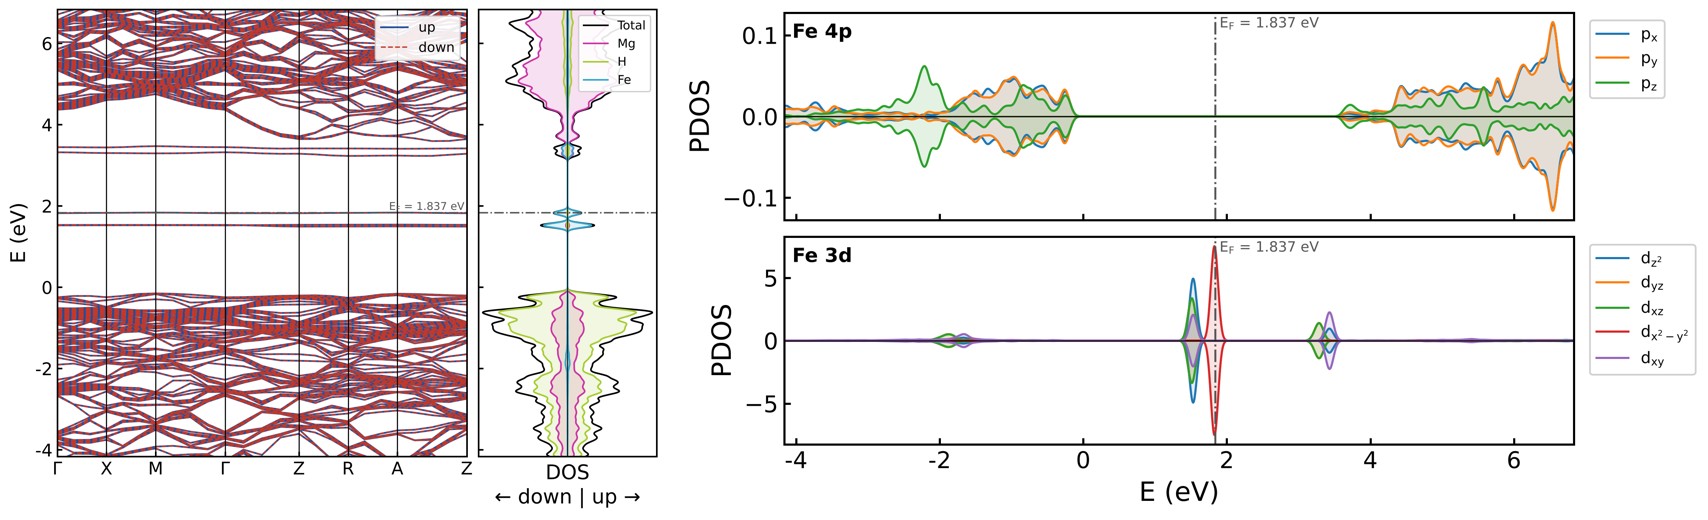
\includegraphics[width=\linewidth]{figures/fermi_python.png}
\caption{MgH$_2$:Fe (CASTEP) produced by the command line: band structure with total and element-projected DOS (left) and Fe~4p/3d $m$-resolved PDOS (right), in the original energy scale with the Fermi level ($\eF=1.837$\,eV) marked by a dash-dotted line.}\label{fig:mgh2}
\end{figure}

\begin{figure}[t]\centering
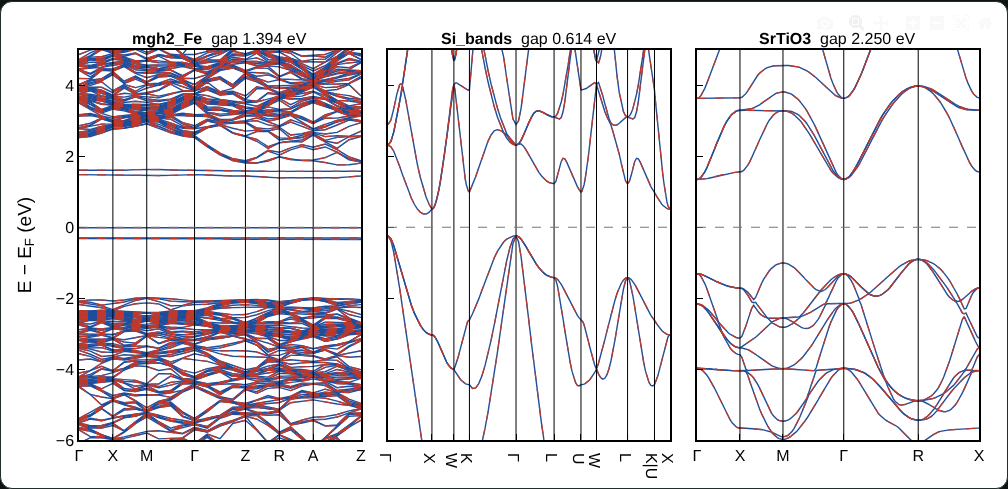
\includegraphics[width=\linewidth]{figures/comparison.png}
\caption{Comparison tab: band structures of calculations from three different codes (CASTEP MgH$_2$:Fe, VASP Si, SIESTA SrTiO$_3$) displayed side by side, each aligned at its own Fermi level.}\label{fig:cmp}
\end{figure}
